\documentclass[10pt]{article}
\usepackage[margin=2.2cm]{geometry}
\usepackage{graphicx}
\usepackage{booktabs}
\usepackage{amsmath}
\usepackage{amssymb}
\usepackage{xcolor}
\usepackage[hidelinks]{hyperref}
\setlength{\parskip}{4pt}
\setlength{\parindent}{0pt}
\graphicspath{{../../../output/02_na_apodization/}}

\title{\vspace{-1.2cm}\textbf{Review 02 --- NA convergence \& apodization}\\
\large \texttt{mcdo\_dev} Phase 2 \quad(\texttt{output/02\_na\_apodization/},
\texttt{docs/theory/02\_apodization\_scalar\_debye.md})}
\author{}
\date{2026-06-12}

\begin{document}
\maketitle
\vspace{-1.1cm}

\section*{Modules and theory chain}

\texttt{apodization.py}: aplanatic Gaussian illumination (sine condition
$r=f\sin\theta$)
$$A(\theta)=\exp\!\Big(-\alpha_t\frac{\sin^2\theta}{\sin^2\alpha}\Big),\qquad
\alpha_t=\Big(\frac{r_{ap}}{w}\Big)^2 \quad \text{[Horv\'ath \& Bor 2003]}$$
\texttt{debye.py}: scalar Debye integral (same $A(\theta)$ and
$\sqrt{\cos\theta}$, vector kernels dropped) + analytic Airy
$[2J_1(v)/v]^2$ and axial $\mathrm{sinc}^2(u/4)$.

\textbf{Chain logic:} RW $-$ scalar isolates \emph{polarization (vector)
effects}; scalar $-$ Airy isolates \emph{wide-angle geometry}. All results at
$\lambda=750$ nm, $n=1.3$, $X_{NA}=n\sin\alpha$.

\section*{Key numbers}

\begin{itemize}\itemsep1pt
\item Low-NA correctness: all theories coincide with Airy to
  $10^{-4}$--$10^{-3}$ at $X_{NA}=0.1$ (check 1).
\item Vector thresholds (uniform): $x$-cut vs scalar exceeds 1\% at
  $X_{NA}\approx0.30$, 5\% at $\approx0.60$; $y$-cut stays $\lesssim2\%$ to
  $\approx0.9$ (check 3) --- threshold statements require polarization + cut.
\item Axial first minimum: $u_0\,4\pi\!\to\!8.98$ and depth
  $10^{-7}\!\to\!10^{-2}$ for $X_{NA}\,0.1\!\to\!1.2$ (check 4).
\item Apodization: $\alpha_t\to0$ regression $=$ uniform to $10^{-13}$;
  FWHM$_v$ 3.17$\,\to\,$4.80 for $\alpha_t$ 0$\,\to\,$4, Airy rings suppressed
  (check 5).
\item Anisotropy $=$ longitudinal field: FWHM$_x$/FWHM$_y\to1.4$ at
  $X_{NA}=1.2$, tracking the $E_z$ energy fraction (check 6).
\item Axial direction (check 7): scalar holds far longer on axis --- uniform
  reaches 1\% only at $X_{NA}\approx1.15$ (never 5\%); the on-axis vector
  ingredient is just the smooth $(1+\cos\theta)$ kernel (no $E_z$, no
  anisotropy). With $\alpha_t{=}4$ the axial deviation grows earlier
  (1\% @ 0.60) --- kernel reweighting moves a soft pupil more than a hard one.
\item Input polarization (check 8; headline results stay linear-$x$):
  circular input gives $|I_0|^2+|I_2|^2+2|I_1|^2$ (no zeros); its thresholds
  are 1\%/5\% at $X_{NA}\approx0.45/0.90$ --- the old report's lenient numbers
  recovered under its (circular) convention.
\item \textbf{Corrected threshold study (reverses the old progress report):}
  with the scalar reference using the \emph{same} $A(\theta)$, Gaussian
  illumination \emph{extends} scalar validity (table below). The report's
  ``Gaussian fails at NA$\approx$0.3'' compared against the paraxial
  Gaussian-beam formula (invalid at high NA); its lenient uniform numbers came
  from circular-polarization averaging. Errata: \texttt{docs/report\_errata.md}.
\end{itemize}

\begin{center}
\small
\begin{tabular}{lccc}
\toprule
illumination & $x$-cut 1\% & $x$-cut 5\% & $x$-dev at $\sin\alpha=0.9$\\
\midrule
uniform & $X_{NA}$ 0.30 & 0.60 & 32.1\%\\
Gaussian $\alpha_t{=}1$ & 0.35 & 0.65 & 25.4\%\\
Gaussian $\alpha_t{=}4$ & 0.40 & 0.85 & \textbf{12.6\%}\\
\bottomrule
\end{tabular}
\end{center}

\clearpage
\begin{center}
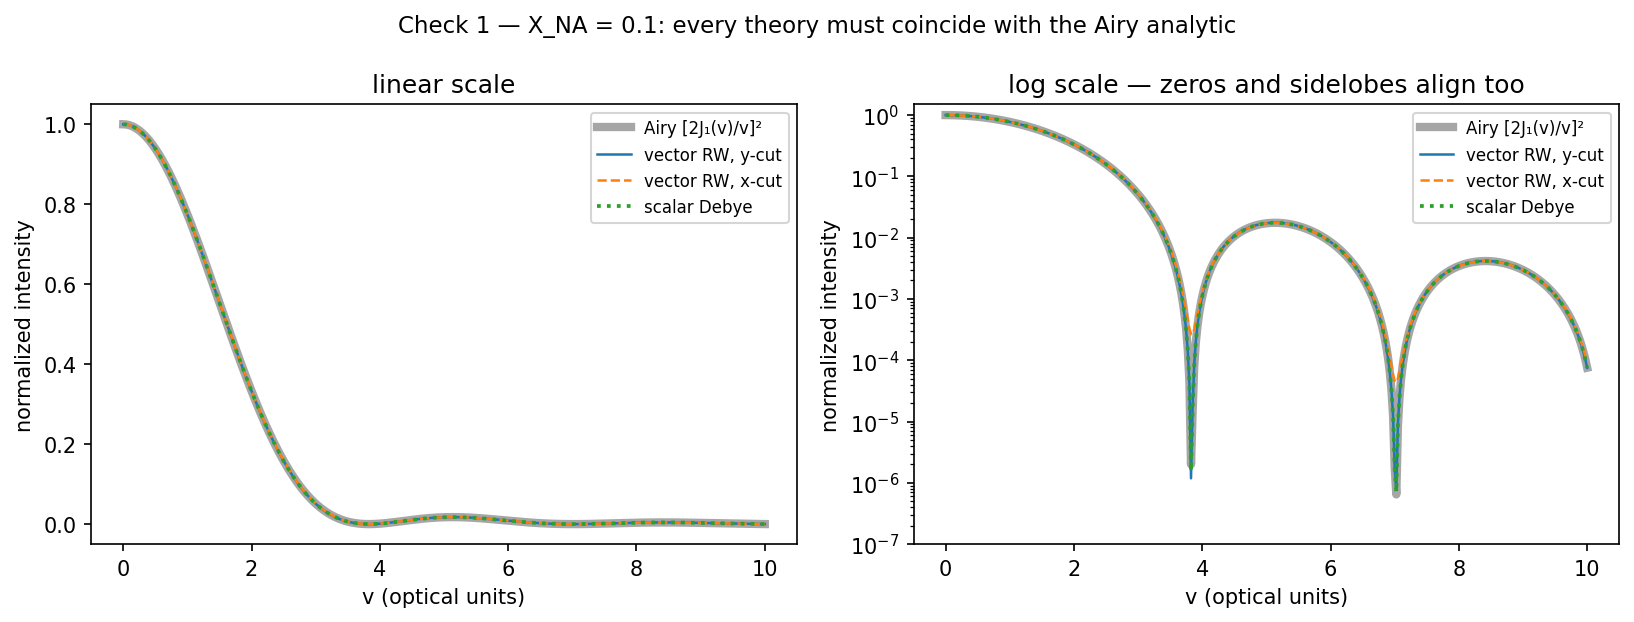
\includegraphics[width=0.92\textwidth]{check1_lowNA_convergence.png}
\end{center}
\textbf{Check 1 (low-NA correctness).} $X_{NA}=0.1$: vector RW (both cuts),
scalar Debye and analytic Airy coincide; the log panel shows zeros and
sidelobes aligned down to $10^{-6}$.

\begin{center}
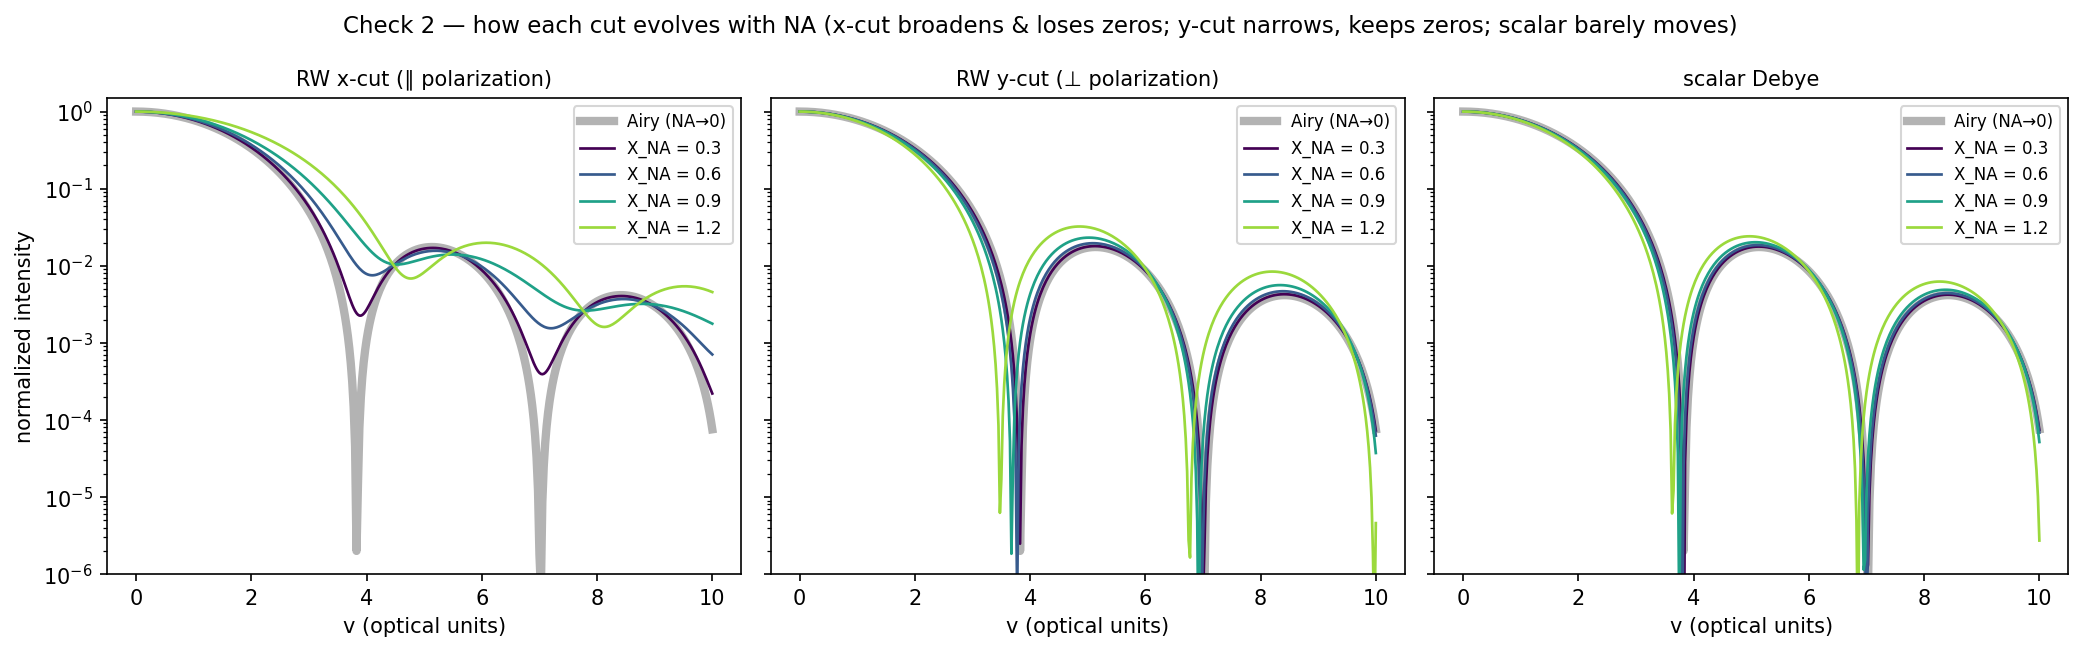
\includegraphics[width=0.98\textwidth]{check2_highNA_vector.png}
\end{center}
\textbf{Check 2 (high-NA behavior).} NA line-families per cut: the $x$-cut's
zeros fill (longitudinal $E_z$) and its lobe broadens with NA; the $y$-cut
narrows and keeps true zeros; scalar barely moves.

\begin{center}
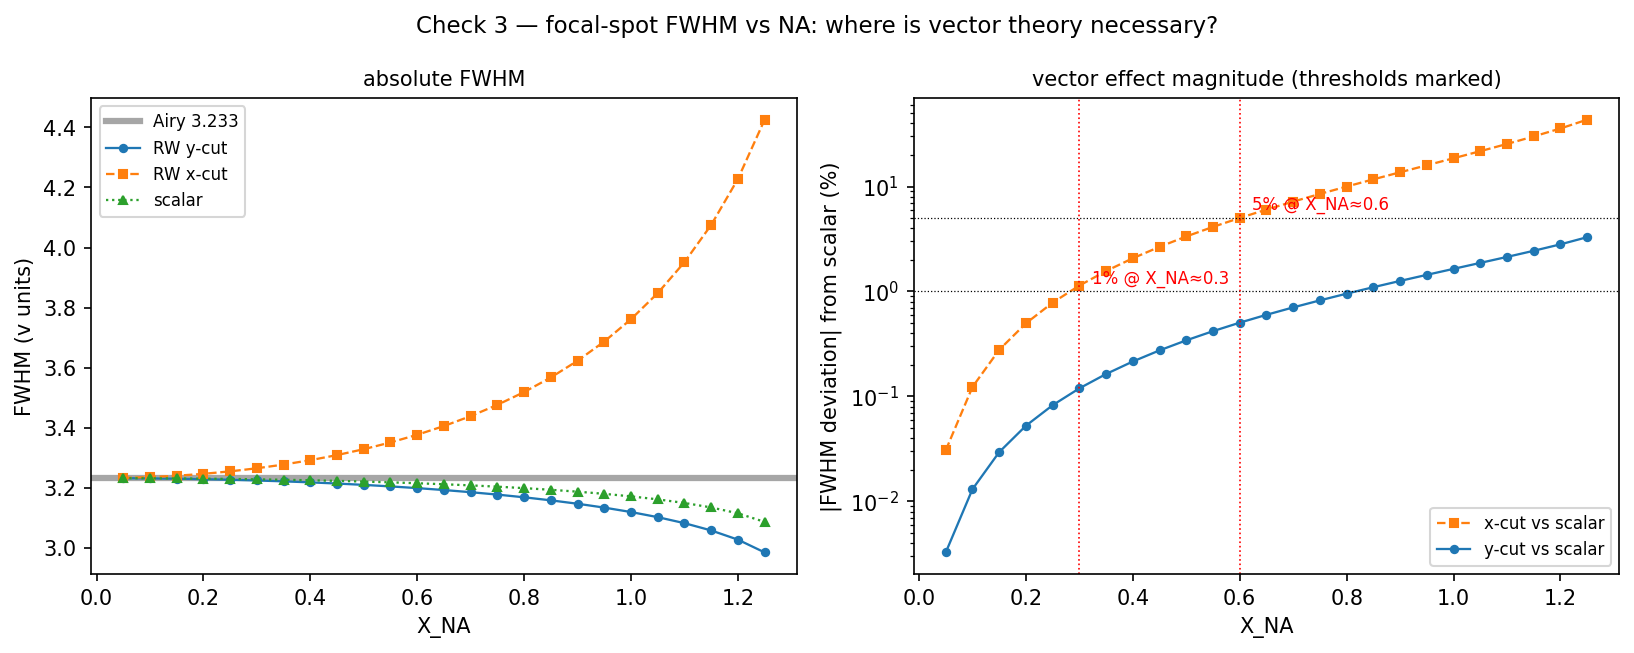
\includegraphics[width=0.95\textwidth]{check3_fwhm_thresholds.png}
\end{center}
\textbf{Check 3 (thresholds, uniform).} FWHM vs NA and \%-deviation with the
1\%/5\% crossings marked at $X_{NA}\approx0.30/0.60$ ($x$-cut).

\clearpage
\begin{center}
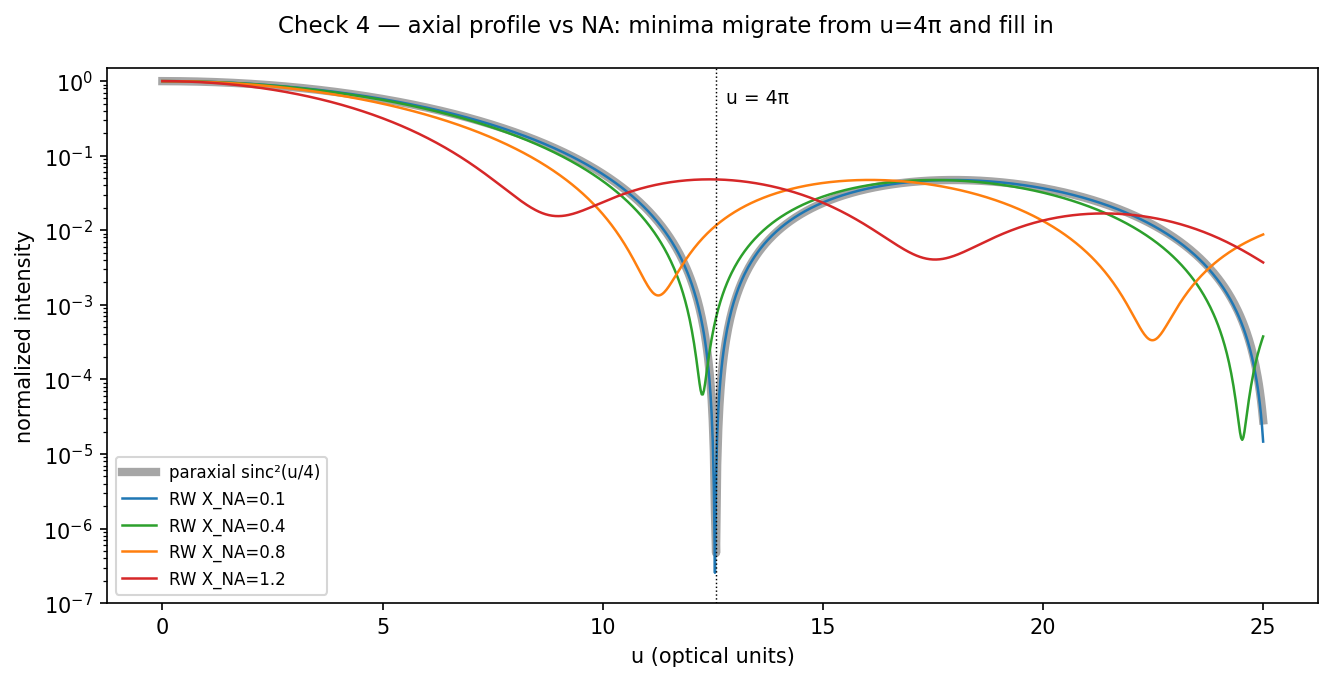
\includegraphics[width=0.62\textwidth]{check4_axial.png}
\end{center}
\textbf{Check 4 (axial).} Minima migrate focus-ward from $u=4\pi$ and fill in
at high NA --- axial zeros are not exact (relevant to optical sectioning).

\begin{center}
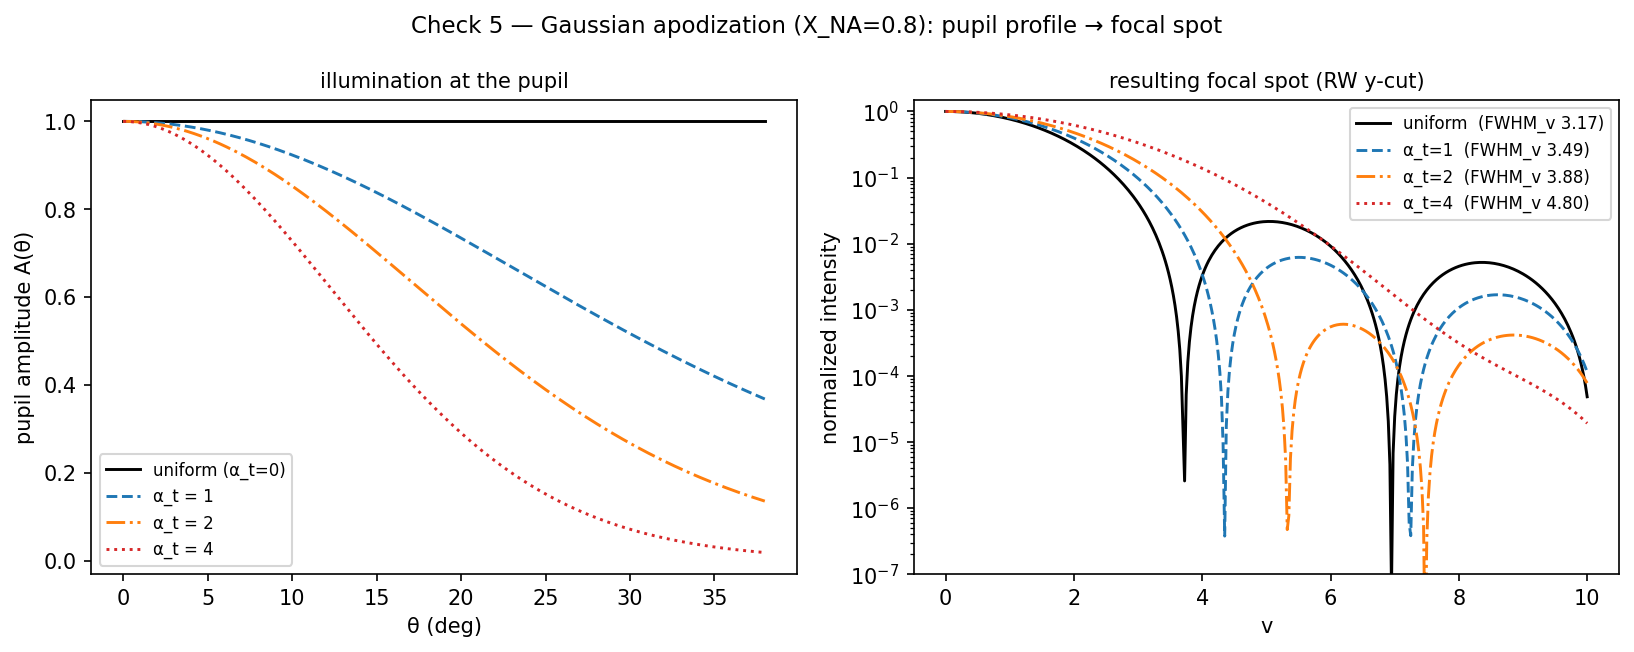
\includegraphics[width=0.92\textwidth]{check5_apodization.png}
\end{center}
\textbf{Check 5 (apodization).} Pupil profile $\to$ focal spot: underfilling
($\alpha_t\uparrow$) broadens the spot and suppresses the hard-edge Airy rings.

\begin{center}
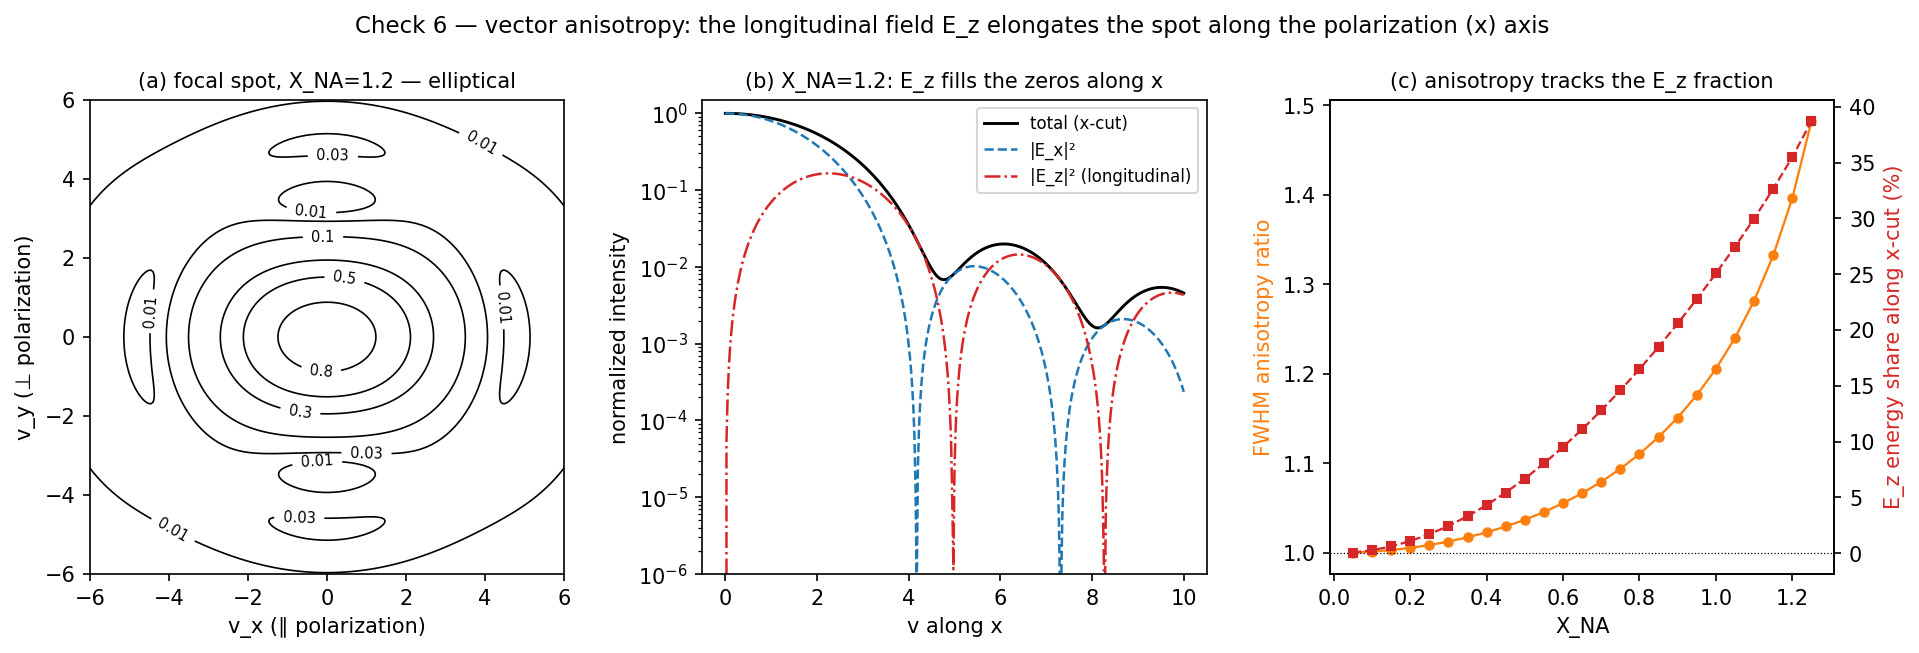
\includegraphics[width=0.98\textwidth]{check6_anisotropy.png}
\end{center}
\textbf{Check 6 (anisotropy).} Elliptical spot at $X_{NA}=1.2$; along $x$ the
longitudinal $|E_z|^2$ fills the $|E_x|^2$ zeros; the FWHM anisotropy ratio
tracks the $E_z$ energy fraction.

\begin{center}
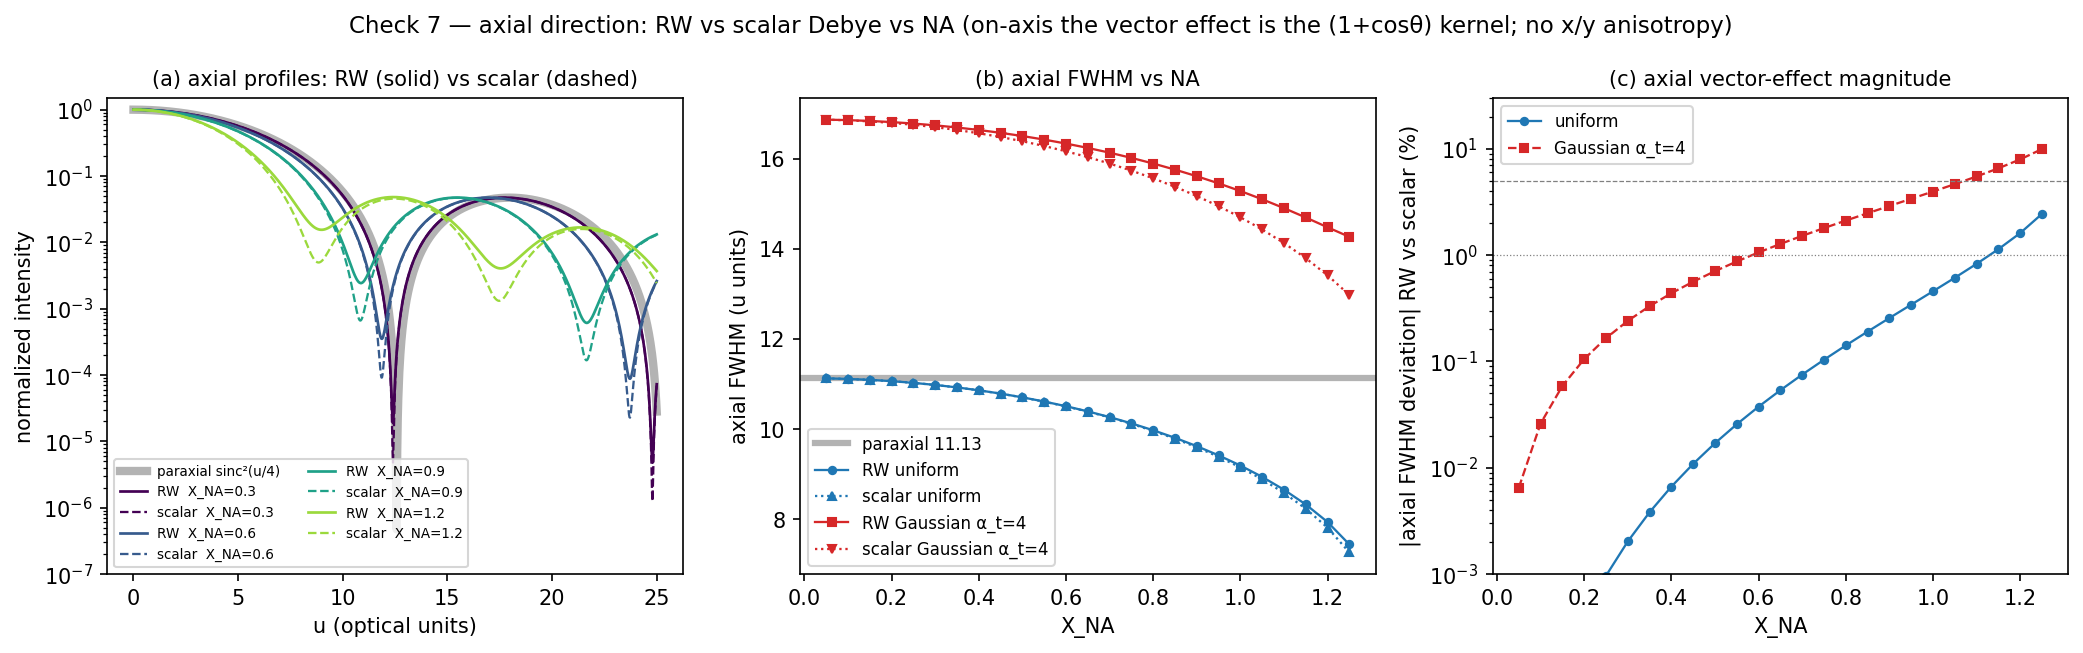
\includegraphics[width=0.98\textwidth]{check7_axial_vs_na.png}
\end{center}
\textbf{Check 7 (axial direction).} RW vs scalar (same $A(\theta)$) along the
axis: profiles per NA (a), axial FWHM vs NA (b), deviation (c). Uniform stays
scalar-accurate to $X_{NA}\approx1.15$ (1\%); Gaussian $\alpha_t{=}4$ crosses
1\% at 0.60. All curves are for a single linearly $x$-polarized input; on axis
the polarization orientation is irrelevant.

\begin{center}
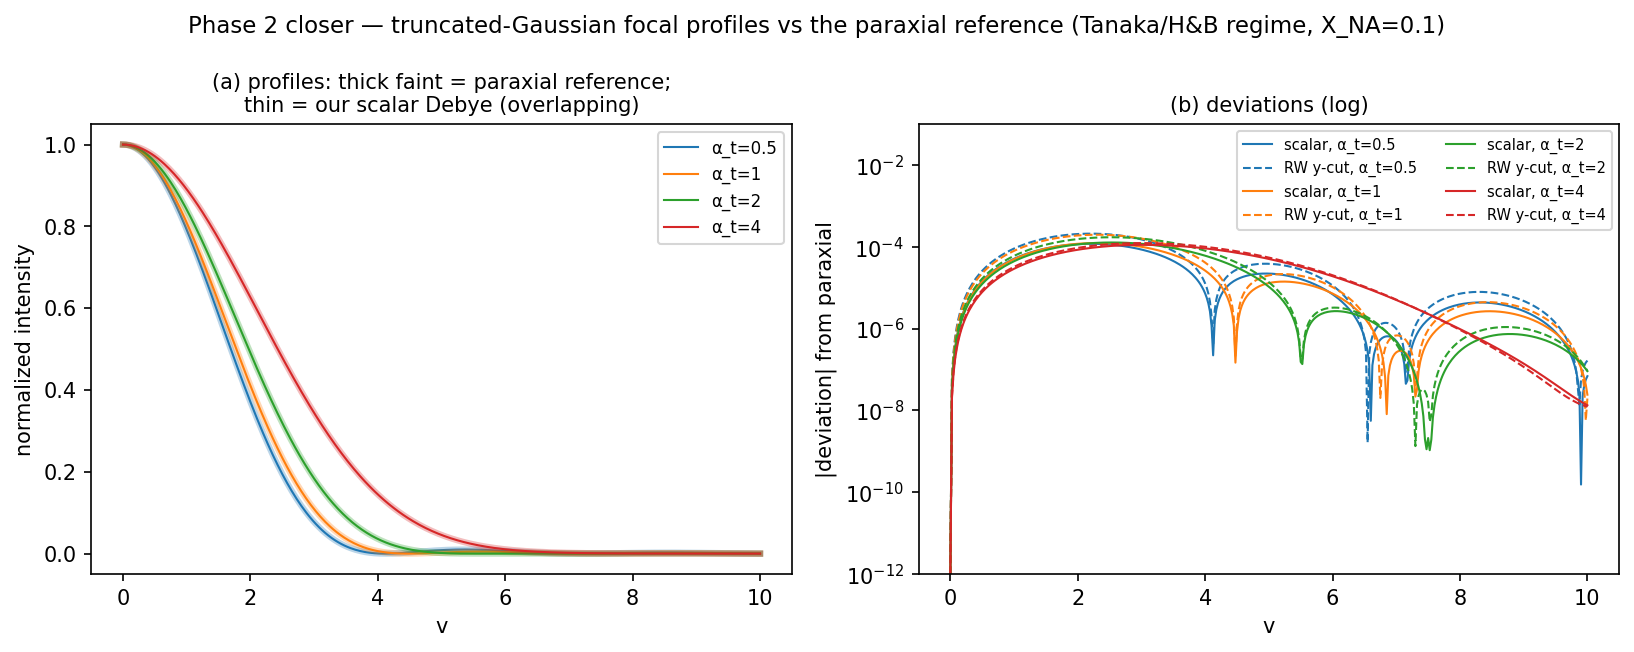
\includegraphics[width=0.95\textwidth]{verify_tanaka_paraxial.png}
\end{center}
\textbf{Closer --- independent paraxial checkpoint.} Truncated-Gaussian focal
profiles vs a direct quadrature of $\int_0^1 e^{-\alpha_t\rho^2}J_0(v\rho)\rho\,d\rho$
(Tanaka 1985 / H\&B regime, no shared code). Our scalar Debye \emph{and} the RW
y-cut match it to $\sim$10$^{-4}$ for $\alpha_t$=0.5--4 at $X_{NA}$=0.1 ---
the apodization is correct against an external reference.

\begin{center}
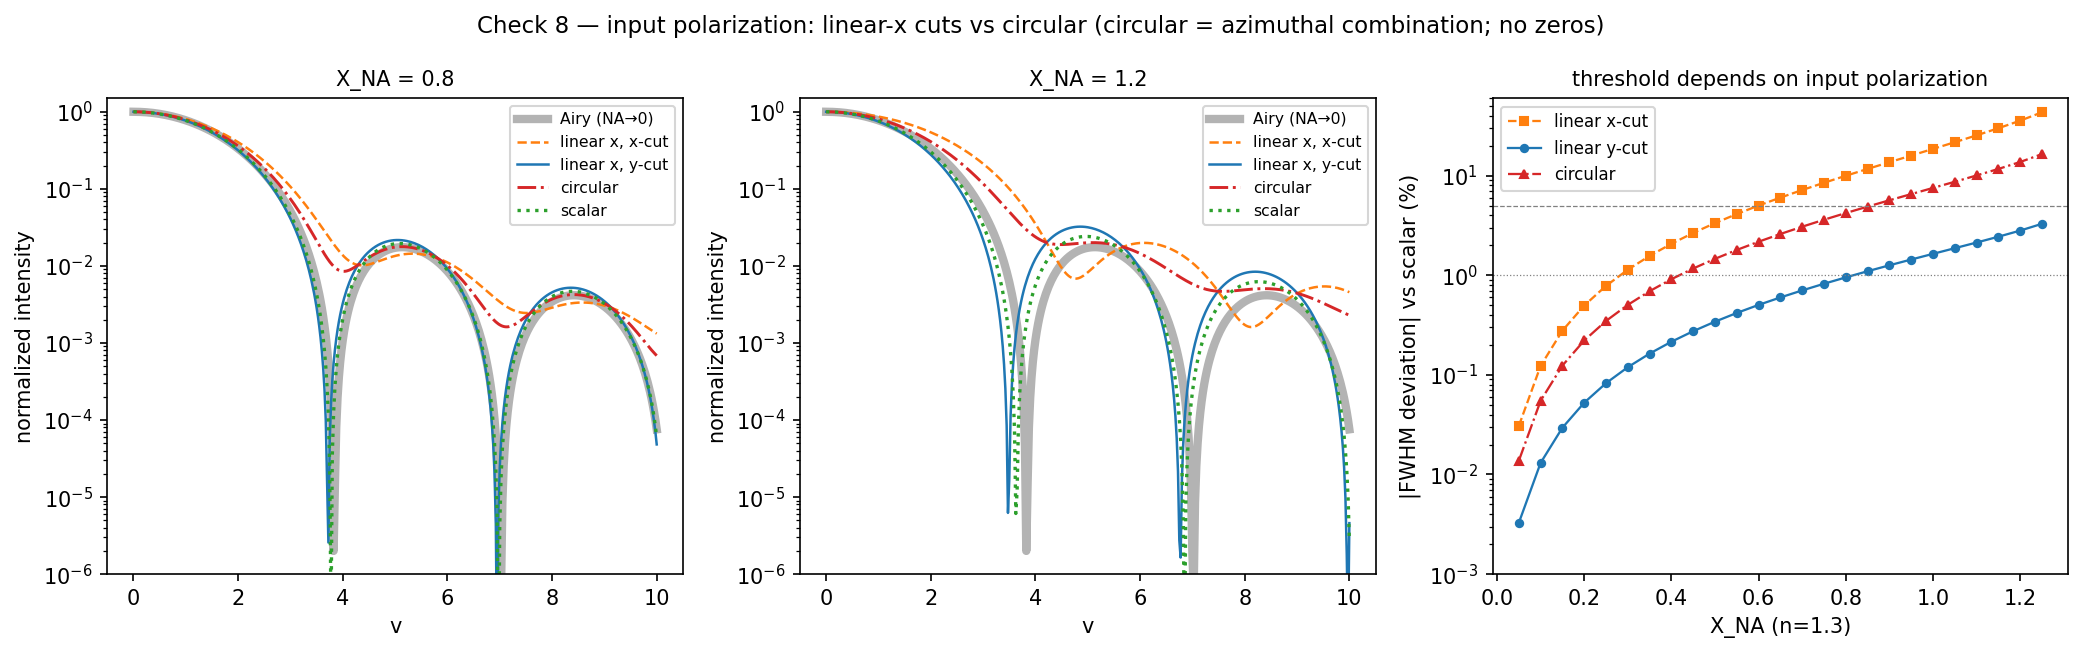
\includegraphics[width=0.98\textwidth]{check8_polarization.png}
\end{center}
\textbf{Check 8 (input polarization).} Linear-$x$ cuts vs circular input vs
scalar at $X_{NA}=0.8$ and $1.2$, and FWHM deviation vs NA per polarization:
thresholds are 0.30/0.60 (linear, $x$-cut), 0.45/0.90 (circular), 0.85/--
(linear, $y$-cut). Circular has no zeros and averages away the anisotropy.

\begin{center}
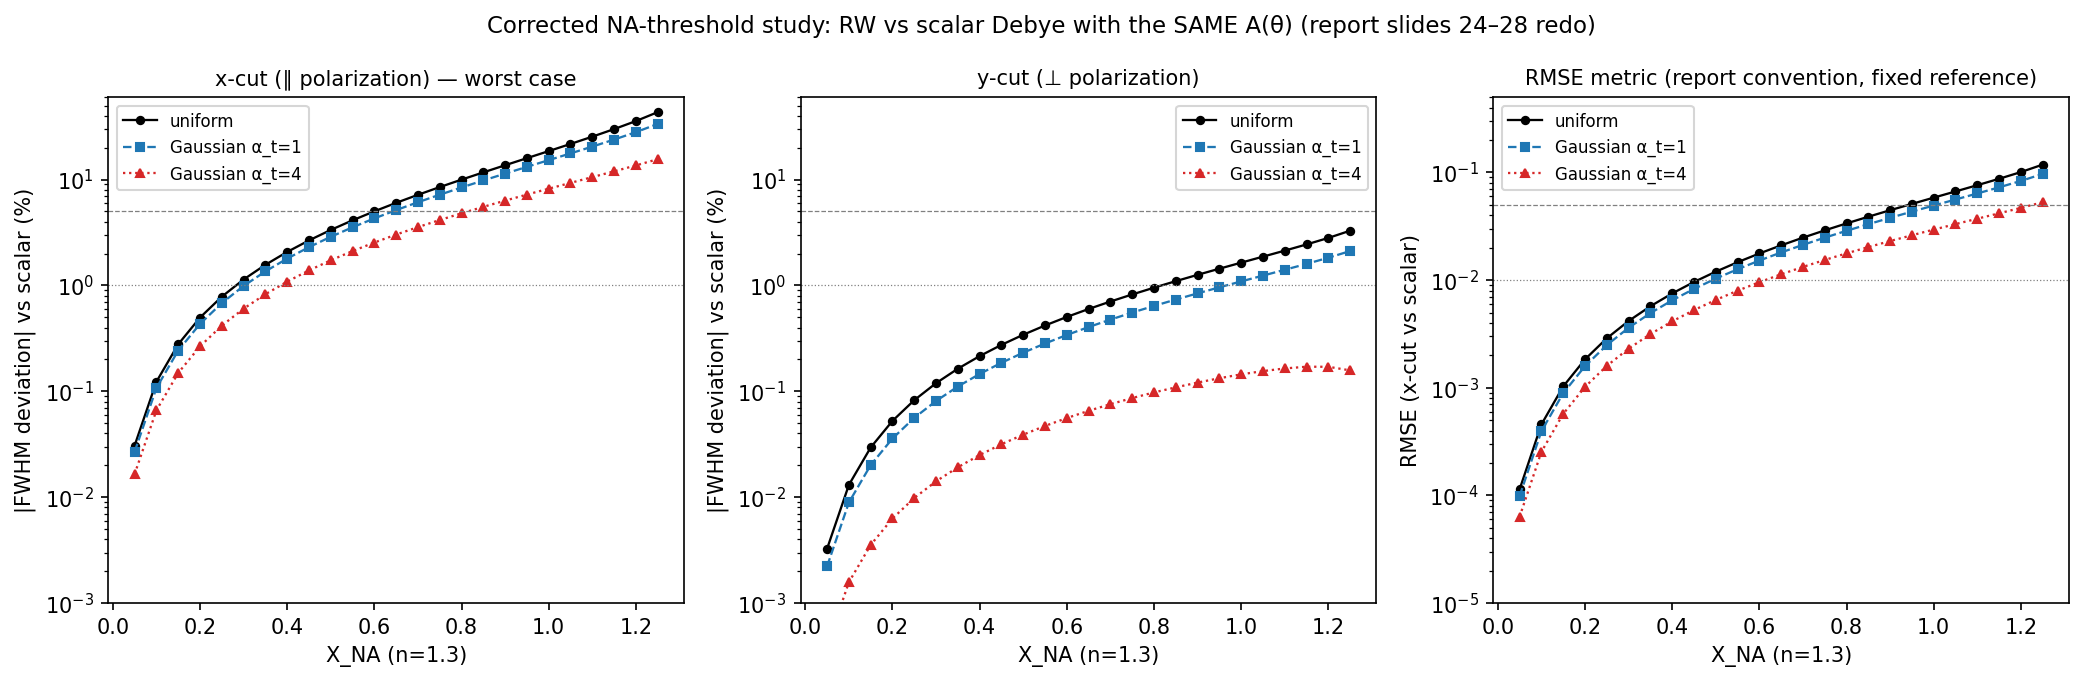
\includegraphics[width=0.98\textwidth]{verify_apod_thresholds.png}
\end{center}
\textbf{Corrected NA-threshold study} (slides 24--28 redo): Gaussian
$\alpha_t{=}4$ sits below uniform in every panel --- $x$-cut, $y$-cut, and the
report's own RMSE metric. Gaussian illumination is \emph{more}
scalar-friendly, not less.

\end{document}
